% Created 2021-10-29 Fri 20:17
% Intended LaTeX compiler: xelatex
\documentclass[letterpaper]{article}
\usepackage{graphicx}
\usepackage{grffile}
\usepackage{longtable}
\usepackage{wrapfig}
\usepackage{rotating}
\usepackage[normalem]{ulem}
\usepackage{amsmath}
\usepackage{textcomp}
\usepackage{amssymb}
\usepackage{capt-of}
\usepackage{hyperref}
\setlength{\parindent}{0pt}
\usepackage[margin=1in]{geometry}
\usepackage{fontspec}
\usepackage{svg}
\usepackage{tikz}
\usepackage{cancel}
\usepackage{pgfplots}
\usepackage{indentfirst}
\setmainfont[ItalicFont = LiberationSans-Italic, BoldFont = LiberationSans-Bold, BoldItalicFont = LiberationSans-BoldItalic]{LiberationSans}
\newfontfamily\NHLight[ItalicFont = LiberationSansNarrow-Italic, BoldFont       = LiberationSansNarrow-Bold, BoldItalicFont = LiberationSansNarrow-BoldItalic]{LiberationSansNarrow}
\newcommand\textrmlf[1]{{\NHLight#1}}
\newcommand\textitlf[1]{{\NHLight\itshape#1}}
\let\textbflf\textrm
\newcommand\textulf[1]{{\NHLight\bfseries#1}}
\newcommand\textuitlf[1]{{\NHLight\bfseries\itshape#1}}
\usepackage{fancyhdr}
\usepackage{csquotes}
\pagestyle{fancy}
\usepackage{titlesec}
\usepackage{titling}
\makeatletter
\lhead{\textbf{\@title}}
\makeatother
\rhead{\textrmlf{Compiled} \today}
\lfoot{\theauthor\ \textbullet \ \textbf{2021-2022}}
\cfoot{}
\rfoot{\textrmlf{Page} \thepage}
\renewcommand{\tableofcontents}{}
\titleformat{\section} {\Large} {\textrmlf{\thesection} {|}} {0.3em} {\textbf}
\titleformat{\subsection} {\large} {\textrmlf{\thesubsection} {|}} {0.2em} {\textbf}
\titleformat{\subsubsection} {\large} {\textrmlf{\thesubsubsection} {|}} {0.1em} {\textbf}
\setlength{\parskip}{0.45em}
\renewcommand\maketitle{}
\author{Houjun Liu}
\date{\today}
\title{MVC PS\#15}
\hypersetup{
 pdfauthor={Houjun Liu},
 pdftitle={MVC PS\#15},
 pdfkeywords={},
 pdfsubject={},
 pdfcreator={Emacs 28.0.50 (Org mode 9.4.4)}, 
 pdflang={English}}
\begin{document}

\tableofcontents


\section{Diff. in Lots of Dims. Worksheet}
\label{sec:orgde24e60}
\subsection{Derivative Matrix of \(f(x,y) = xy\ln(xy)\)}
\label{sec:org138f1f6}
The derivative matrix of the function \(f(x,y) = xy\ln(xy)\) is \(\nabla f(x,y) = xy\ln(xy)\) and therefore is: 

\begin{equation}
\begin{bmatrix}
y \ln(xy) \\
x \ln(xy)
\end{bmatrix}
\end{equation}

\subsection{Derivative matrix of \(f(t) = t^5 \hat{i} - 2t \hat{j} + t^2 \hat{k}\)}
\label{sec:org1e30235}

The derivative matrix of the function \(f(t) = t^5 \hat{i} - 2t \hat{j} + t^2 \hat{k}\) is: 

\begin{equation}
\begin{bmatrix}    
5t^4 \\
-2 \\
2t \\
\end{bmatrix}    
\end{equation}


\subsection{Classmates' Partial Derivative}
\label{sec:orgaf7b151}
\begin{quote}
Suppose that one of your classmates reports that for a particular function \(f(x,y)\), the partial derivatives are:

\begin{equation}
    \frac{\partial f}{\partial x} = 2x+3y
\end{equation}

\begin{equation}
    \frac{\partial f}{\partial x} = 4x+6y
\end{equation}

Do you believe them?
\end{quote}

No, I do not. Partial derivatives with both variables in \emph{both} partials shouldn't result in both variables existing in the 1st-degree: if, say, one variable were to exist in the first degree in one case, it would be completely eliminated in the other as it is constant. 

Hence, I do not believe this function exist.

\subsection{Partial derivatives from \(\mathbb{R}^n\) to \(\mathbb{R}^m\)}
\label{sec:org984614d}
For first partial derivatives from \(\mathbb{R}^n \to \mathbb{R}^m\), given the shape of the derivative matrix corresponding to this transformation, would have \(n\times m\) partial derivatives.

Based on the patterns of repetition for the input variables, the second partial derivative would have \(n \times n \times m\) entries --- as per each new partial, there is \(n \times n\) combinations of the two input dimensions. 

\section{Roofs Problem 1}
\label{sec:org25d1bcb}
\subsection{Picture of the Situation}
\label{sec:orgba6d205}

\begin{center}
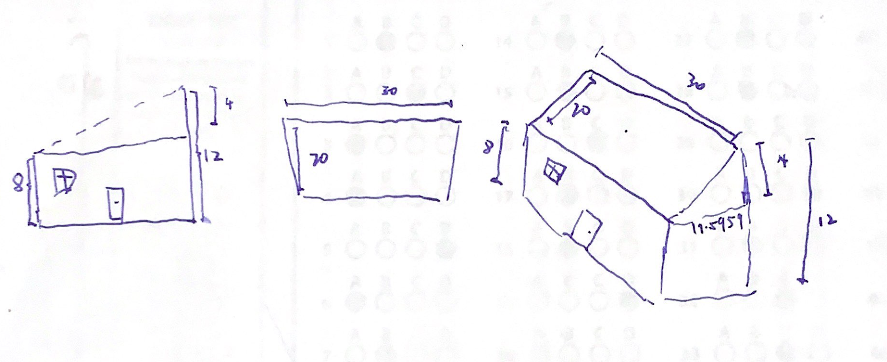
\includegraphics[width=.9\linewidth]{2021-10-29_20-16-14_screenshot.png}
\end{center}


\subsection{Function for the Roof}
\label{sec:org02c90f6}
As the roof does not curve except in one edge, the function of the roof could be written as:

\begin{equation}
f(x,y) = \frac{1}{2\sqrt{6}}y \{0\leq x \leq 30, 0 \leq y \leq 8\sqrt{6}\}
\end{equation}

\subsection{Slope of the roof, looking up}
\label{sec:org7dae934}
Standing on the center of the roof, looking at the tall side, the slope of the roof is the "slope" of the function: \(\frac{1}{2\sqrt{6}}\). 

The no-calculus result for this is simply the ratio between the "height" side (\(4ft\)) and the "bottom" side (\(8\sqrt{6} = \sqrt{384}\)): \(\frac{1}{2\sqrt{6}}\).

With calculus, this is equally as simple. The gradient of \(f\) could be represented as:

\begin{equation}
    \begin{bmatrix}
0 \\
\frac{1}{2\sqrt{6}}
    \end{bmatrix}
\end{equation}

Standing in the center, looking on the tall side, we are facing the direction "up" the \(y\) axis:

\begin{equation}
    \begin{bmatrix}
0 \\
1
    \end{bmatrix}
\end{equation}

The dot product between the two vectors, as we expect, is the same value as the no-calculus result:

\begin{equation}
     \begin{bmatrix}
0 \\
\frac{1}{2\sqrt{6}}
    \end{bmatrix}
\cdot
    \begin{bmatrix}
0 \\
1
    \end{bmatrix} = \frac{1}{2\sqrt{6}}
\end{equation}

This represents an angle of roughly \(11.5^{\circ}\).

\subsection{Slope of the roof, looking to the side}
\label{sec:org98b9694}
Looking to the side, you are not facing an incline of the roof. Hence, the intuitive answer is that the slope of the roof is \(0\).

Leveraging the same line of mathematics, we could figure the same slope as described above:

\begin{equation}
     \begin{bmatrix}
0 \\
\frac{1}{2\sqrt{6}}
    \end{bmatrix}
\cdot
    \begin{bmatrix}
1 \\
0
    \end{bmatrix} = 0
\end{equation}

This, of course, also represents \(0^{\circ}\).

\subsection{Slope of the roof, looking towards a corner}
\label{sec:orgbf53d26}
The middle of the board is located at \((15, 4\sqrt{6})\). We are facing now the location \((30, 8\sqrt{6})\). Therefore, the vector of our sight could be represented as \((15, 4\sqrt{6})\).

The magnitude of this vector is \(\sqrt{321} \approx 17.92\); hence, the normalized vector is \((\frac{15}{\sqrt{321}}, \frac{4 \sqrt{6}}{\sqrt{321}})\)

Creating a dot product of the gradient and this result direction vector, result in:

\begin{equation}
     \begin{bmatrix}
0 \\
\frac{1}{2\sqrt{6}}
    \end{bmatrix}
\cdot
    \begin{bmatrix}
\frac{15}{\sqrt{321}}\\
\frac{4 \sqrt{6}}{\sqrt{321}}
    \end{bmatrix} = \frac{2}{\sqrt{321}}
\end{equation}

This represents an angle of roughly \(6.4^{\circ}\).
\end{document}
